\documentclass{journal}

\usepackage{multicol}
\usepackage{amsmath}
\usepackage{graphicx}
\usepackage{float}
\usepackage{enumitem}

\title{PID Control of a Robot Via Position Feedback}
\author{Nick Pham}

\begin{document}
%\begin{multicols}{2}

\maketitle

\section*{Setup and Procedure}

Please refer to the lab handout for this information.

\section*{Prelab}
\begin{enumerate}[label=(\alph*)]
	\item % Part a
	The simulink model is a typical feedback controller.  The plant is the state space model described in the lab specification:

	\begin{align}
		\dot{s} &= v \\
		\dot{v} &= -av + bu
	\end{align}

	The velocity plus noise is measured at the A-D converter, which is then added to the desired reference signal and input into the controller.  This is a PID controller, which uses a linear combination of the proportional, integral, and derivative of the error to determine the control input signal to the plant.

	\item % Part b
	The initial values for the coefficients were $K_p = 100$, $K_i = 20$, and $K_d = 0.3$.  This produced an underdamped output for a few seconds before settling to the desired speed (see Figure \ref{fig:PID_100_20_03}).

	\begin{figure}[H]
		\centering
		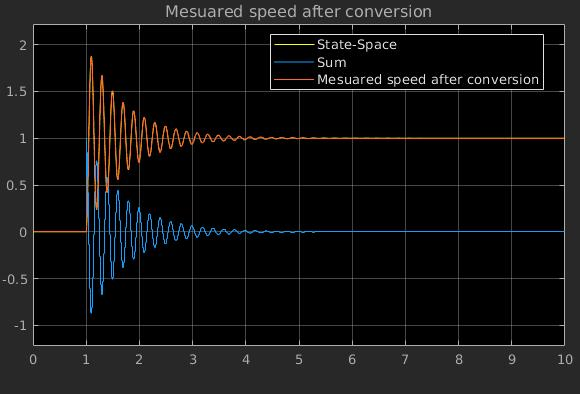
\includegraphics[width = 0.8\textwidth]{Lab1PID_100_20_0point3.jpg}
		\caption{Underdamped response for $K_p = 100$, $K_i = 20$, and $K_d = 0.3$.}
		\label{fig:PID_100_20_03}
	\end{figure}

	Increasing the derivative component $K_d$ to 10 quickly reduces the oscillations (see Figure \ref{fig:PID_100_20_10}).  Because the "strength" of the derivative part of the control was increased, there was a strong corrective action during the high acceleration phase, resulting in much less overshoot and stability in less than a second.

	\begin{figure}[H]
		\centering
		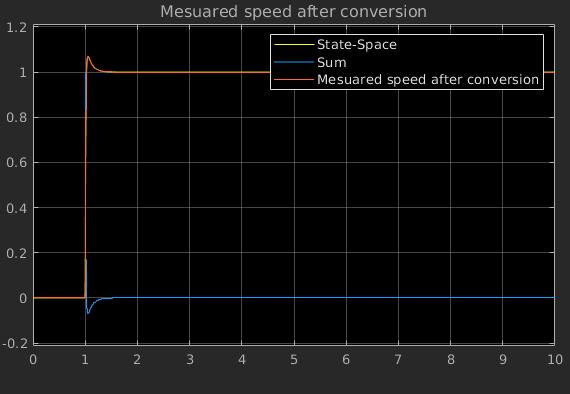
\includegraphics[width = 0.8\textwidth]{Lab1PID_100_20_10.jpg}
		\caption{System response for $K_p = 100$, $K_i = 20$, and $K_d = 10$.}
		\label{fig:PID_100_20_10}
	\end{figure}

	Not all combinations of coefficients result in a successful and stable system.  For intance, removing the proportional control coefficient altogether results in wild and increasing oscillations (see Figure \ref{fig:PID_0_20_03}).  Notice that after 20 seconds, the oscillations grow on the order of $10^{16}$ times the desired speed.

	\begin{figure}[H]
		\centering
		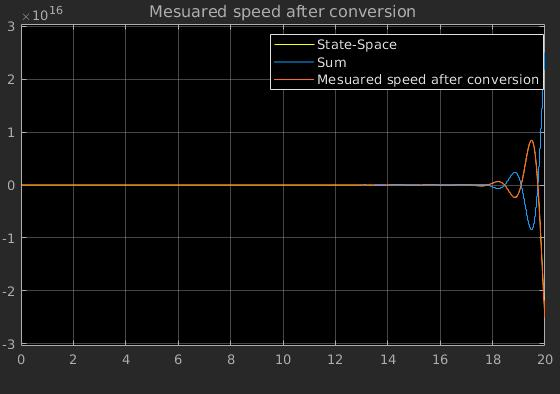
\includegraphics[width = 0.8\textwidth]{Lab1PID_0_20_0point3.jpg}
		\caption{Oscillatory response for $K_p = 0$, $K_i = 20$, and $K_d = 0.3$.}
		\label{fig:PID_0_20_03}
	\end{figure}

	\item % Part c
	To choose these parameters, first find a good $k_p$ value for minimal disturbance.  Then, choose a $k_d$  and $k_i$ values to help find a faster convergence without too much overshoot or oscillations.

	\item % Part d
	The PID auto tuner can be used to set the PID coeffcients for various response times and transient behaviors.  For high performance (response time set to 0.01 seconds and transient behavior set to 0.9), the tuner gave parameters $K_p = 140$, $K_i = 245$, and $K_d = 20$.  This behavior has only a $3.5\%$ overshoot.  This gave fairly similar performance characteristics to the set of coefficients used in Figure \ref{fig:PID_100_20_10}, fast setting with some small overshoot.

	\item % Part e
	Adding noise to the measurement resulted in similar noise in the output when using the settings from the auto tuner (see Figure \ref{fig:Lab1PID_var0.01}).  This probably resulted from the very fast response time, so the output was following the noise accurately.  To improve the quality of the output, the PID controller should filter the signal to remove the noise.  Because the mean of the noise is still 0, a low pass filter could perform this task, which would be implemented by increasing the relative importance of the integration coefficient $K_i$.

	\begin{figure}[H]
		\centering
		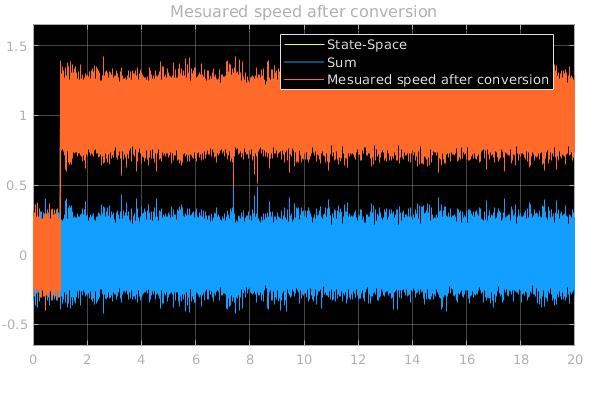
\includegraphics[width = 0.8\textwidth]{Lab1PID_0var01.jpg}
		\caption{System response with auto tuned parameters $K_p = 140$, $K_i = 245$, and $K_d = 20$ to noisy input with $var = 0.01$}
		\label{fig:Lab1PID_var0.01}
	\end{figure}

	\item % Part f
	The sample rate of the measurement also has an important effect on the response of the system.  Decreasing the sample time from 0.0001 to 0.005 results in larger overshoot (see Figure \ref{fig:Lab1PID_sr0.005}).  Decreasing the sample time further to 0.01 results in unstable oscillations (see Figure \ref{fig:Lab1PID_sr0.01}).

	\begin{figure}[H]
		\centering
		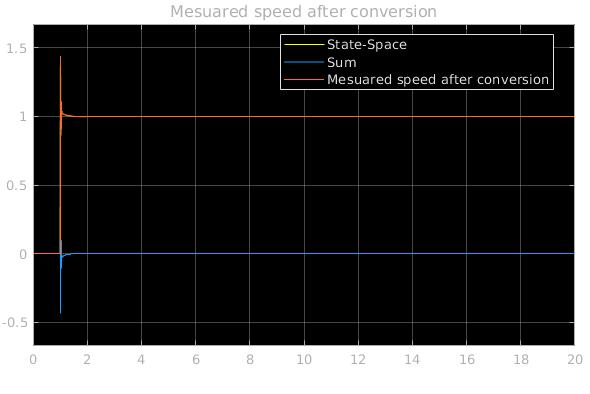
\includegraphics[width = 0.8\textwidth]{Lab1PID_0SR005.jpg}
		\caption{System response with auto tuned parameters $K_p = 140$, $K_i = 245$, and $K_d = 20$ with sample rate limited to 0.005.  Note the large overshoot.}
		\label{fig:Lab1PID_sr0.005}
	\end{figure}

	\begin{figure}[H]
		\centering
		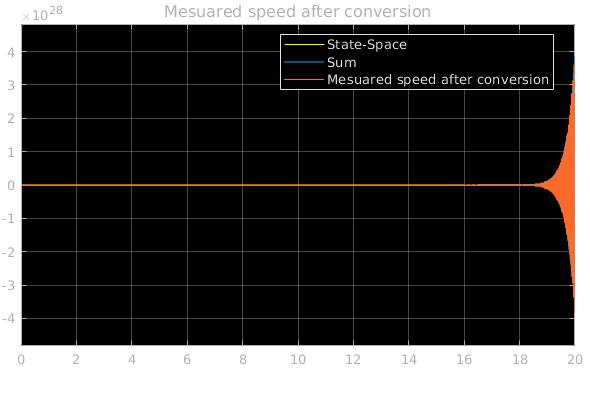
\includegraphics[width = 0.8\textwidth]{Lab1PID_0SR01.jpg}
		\caption{Unstable system response with auto tuned parameters $K_p = 140$, $K_i = 245$, and $K_d = 20$ with sample rate limited to 0.01}
		\label{fig:Lab1PID_sr0.01}
	\end{figure}

	\item % Part g
	To further illustrate the effects of response time on the performance of the system, a sinusoidal input can be used in place of the step input.  Reseting the sample time back to 0.0001, at relatively low frequencies such as $6.3 rad/sec = 1 Hz$, the output tracks the input wave closely, with error on the order of $10^{-2}$ (see Figure \ref{fig:Lab1PID_1Hz}).  However, increasing the frequency of the reference sine wave to $100Hz$ resulted in error on the order of $10^0$, which is about the same amplitude as the reference sine wave itself (see Figure \ref{fig:Lab1PID_100Hz}.

	\begin{figure}[H]
		\centering
		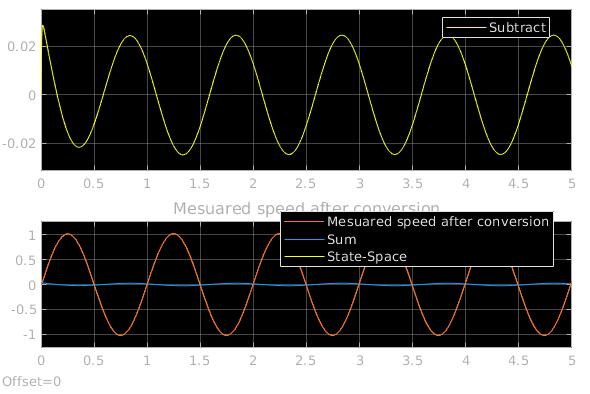
\includegraphics[width = 0.8\textwidth]{Lab1PID_1Hz.jpg}
		\caption{System response with auto tuned parameters $K_p = 140$, $K_i = 245$, and $K_d = 20$ to sinusoidal reference input with frequency $1Hz$.  The uppper plot shows the error signal, on the order of $10^{-2}$.}
		\label{fig:Lab1PID_1Hz}
	\end{figure}

	\begin{figure}[H]
		\centering
		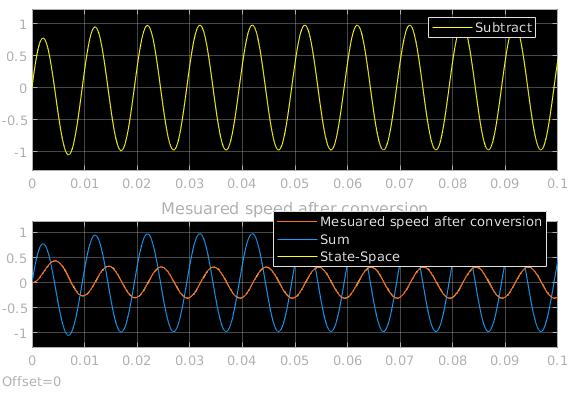
\includegraphics[width = 0.8\textwidth]{Lab1PID_100Hz.jpg}
		\caption{System response with auto tuned parameters $K_p = 140$, $K_i = 245$, and $K_d = 20$ to sinusoidal reference input with frequency $1Hz$.  Note the much larger error signal.}
		\label{fig:Lab1PID_100Hz}
	\end{figure}


\end{enumerate}

\section*{Lab Results and Discussion}
Tuning the PID started with finding a suitable $k_p$ coefficient.  On the suggestion that the range [2, 5] would be a good place to start, the first test was for $(k_p, k_i, k_d) = (2, 0, 0)$.  Figure \ref{fig:Lab1_p2i0d0} shows the system measurements for these values.  Note that the initial condition of the robot was below 0, so the graph is shifted in time somewhat.  With this value, there was some overshoot, but little oscillations.  The PWM of the motor did clip though.

\begin{figure}[H]
	\centering
	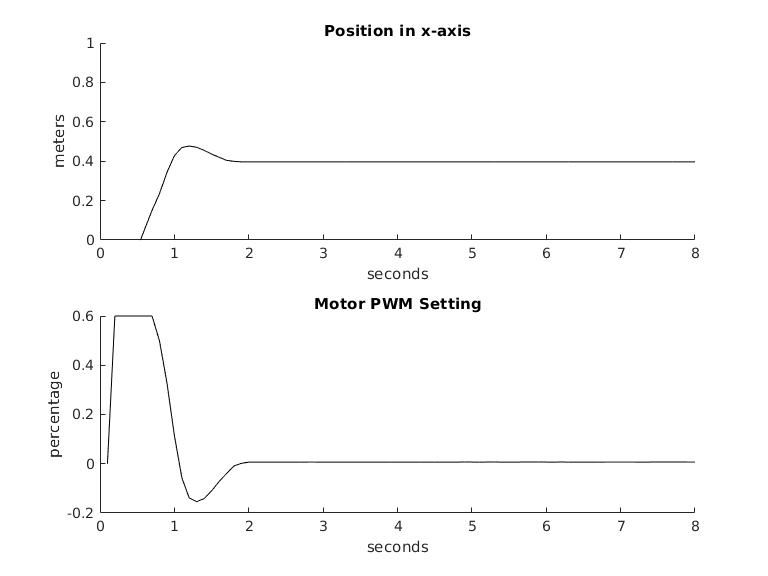
\includegraphics[width = 0.8\textwidth]{NickPhamgraphs/p2i0d0.jpg}
	\caption{System response to $(k_p, k_i, k_d) = (2, 0, 0)$.}
	\label{fig:Lab1_p2i0d0}
\end{figure}

Increasing $k_p$ to 3.5 increased the overshoot and hence oscillations, as seen in Figure \ref{fig:Lab1_p3_5i0d0}.  The graph shows that there may have been some error, as there were some blips a few seconds after the system seemed to settle.

\begin{figure}[H]
	\centering
	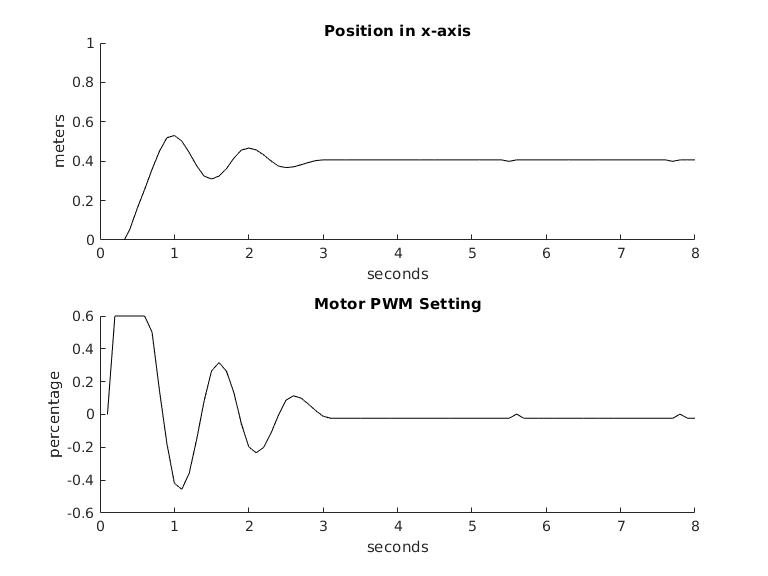
\includegraphics[width = 0.8\textwidth]{NickPhamgraphs/p3_5i0d0.jpg}
	\caption{System response to $(k_p, k_i, k_d) = (3.5, 0, 0)$.}
	\label{fig:Lab1_p3_5i0d0}
\end{figure}

To reduce constant error, the $k_i$ parameter was increased to 1.  Figure \ref{fig:Lab1_p2i1d0} shows the result, which does not converge as well as the just proportional controller.  This might be because the integral part is outweighing the proportional control.  For best results, it is usually good to keep the integral and proportional coefficients much less than the proportional control.

\begin{figure}[H]
	\centering
	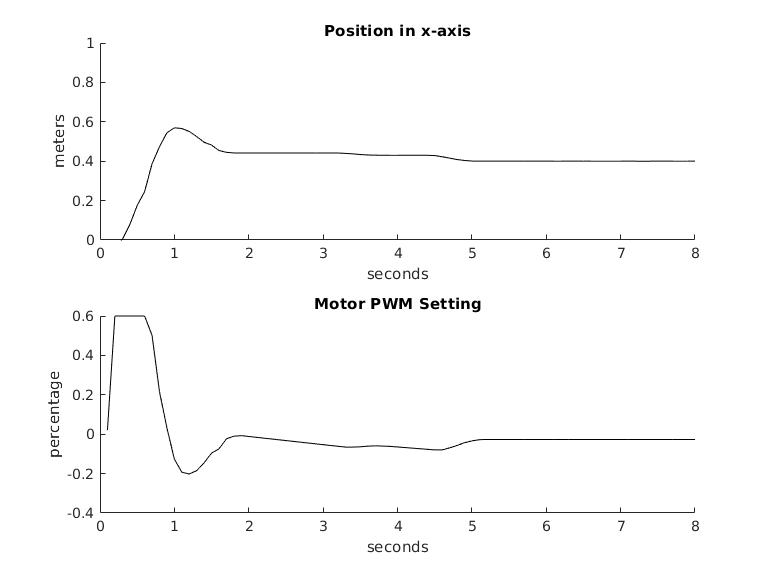
\includegraphics[width = 0.8\textwidth]{NickPhamgraphs/p2i1d0.jpg}
	\caption{System response to $(k_p, k_i, k_d) = (2, 1, 0)$.}
	\label{fig:Lab1_p2i1d0}
\end{figure}

Decreasing the $k_i$ parameter to 0.05 and increase the proportional control to 4 allowed the system to converge, but still with some oscillations, as seen in Figure \ref{fig:Lab1_p4i0_05d0}.

\begin{figure}[H]
	\centering
	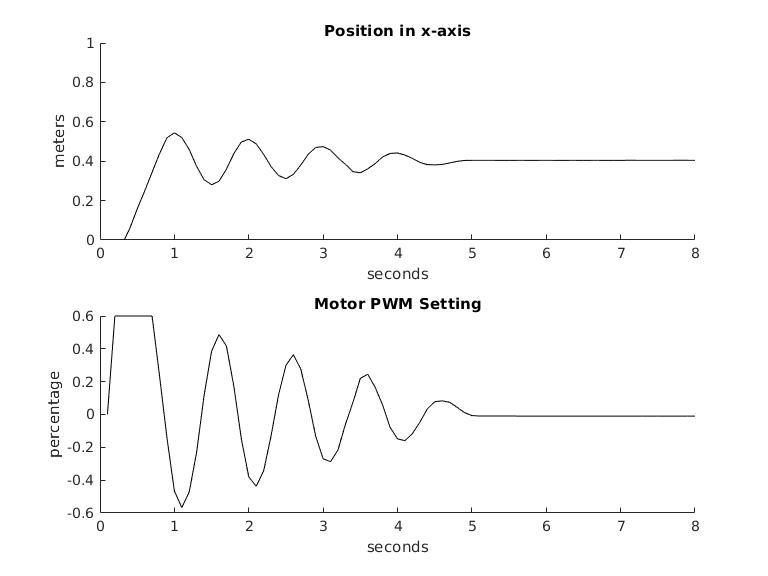
\includegraphics[width = 0.8\textwidth]{NickPhamgraphs/p4i0_05d0.jpg}
	\caption{System response to $(k_p, k_i, k_d) = (4, 0.05, 0)$.}
	\label{fig:Lab1_p4i0_05d0}
\end{figure}

Finally, a derivative control was also included to encourage faster convergence, as seen in Figure \ref{fig:Lab1_p2_5i0_05d0_1}.  However, this was not much if at all better than just the proportional control.  Though in idealized simulations PID controllers do work better than just proportional controls, in the real world with noisy and imprecise measures and non ideal actuators (the motors likely required a certain threshold power to make the vehicle move), a proportional only controller can be sufficient in many cases.

\begin{figure}[H]
	\centering
	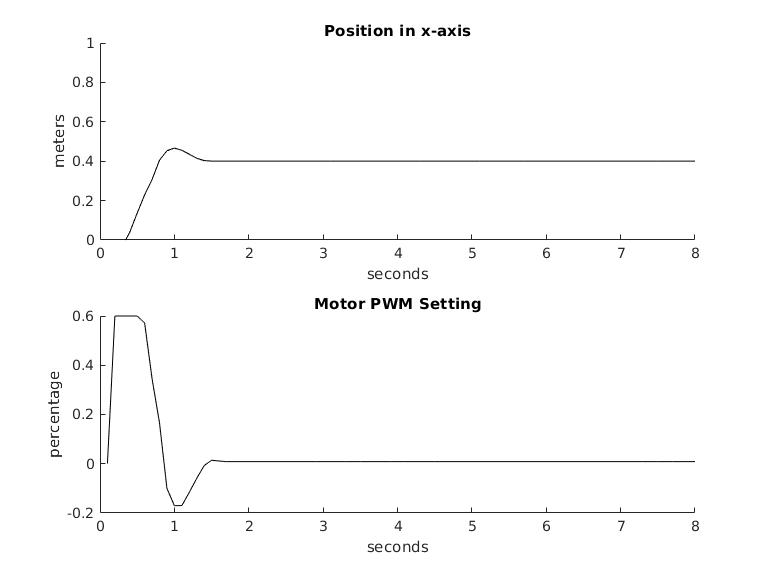
\includegraphics[width = 0.8\textwidth]{NickPhamgraphs/p2_5i0_05d0_1.jpg}
	\caption{System response to $(k_p, k_i, k_d) = (2.5, 0.05, 0.1)$.}
	\label{fig:Lab1_p2_5i0_05d0_1}
\end{figure}

In summary, the $k_p$ parameter increases the feedback control input when the error between the system output and the desired output is large.  This should be the main component of the control.  Large $k_p$ values likely require large resources, so there is an upper bound on this value in practice.  However, larger values of $k_p$ will lead to reaching the target faster, but at the cost of higher overshoot.  Lower values will have less overshoot but take longer to reach the target.

The $k_i$ parameter accounts for the integral for the integral of the error, and is used to correct for long term accuracy error offsets.  It can correct for calibration errors in measurement and actuation devices, but should not be too large compared to the proportional parameter.

The $k_d$ parameter can be used to decrease the response time of the system, because at larger rates of change the control input will be increased.  Like the $k_i$ parameter, it should not be too large compared to $k_p$.  Setting $k_i$ and $k_p$ requires iterative trial and error for fine tuning, and the two must be balanced with each other.


%\end{multicols}
\end{document}